\section{Back-end Library}
\label{sec:backend}
%TimerLib
%\textit{Introduktion til hvorfor det er smart at bruge biblioteker frem for at udvikle på ét workspace\\
%(Man kan nemmere teste på et bibliotek hvor man kan lave en test app, frem for at være afhængig af at "main" appen virker)}
The libraries in WOMBAT each control the storage and drawing functionality of the application.
These functionalities have been imported as Android project libraries, because this gives the developer the ability to create an external project and test the library, without being dependent on a working main project.

Furthermore is a benefit that the libraries works like modules which can be changed to handle e.g. OpenGL instead of canvas in the \texttt{DrawLib}.


\subsection{TimerLib}
\label{subsec:TimerLib}
%\textit{Beskrivelse af timerlib, hvad indeholder timerlib, services\\
%Beskrivelse af implementationen af timerlib med kode eksempler}
\texttt{TimerLib} contains the functionality that store and manage all the different objects that WOMBAT uses. The main goal of \texttt{TimerLib} is to provide a set of simple methods and objects which the rest of WOMBAT can use without knowledge of how \texttt{TimerLib} works. This goal is achieved by being strict about visibility of attributes and methods.

\subsubsection{Classes}
The \texttt{TimerLib} classes are described in the following.

\begin{description}
  \item[Guardian] \hfill \\
  The \texttt{Guardian} class is an object that represent the guardian in our system. The idea of the GIRAF system is that only one guardian can be logged in at a given time, that is why the \texttt{Guardian} class use a singleton pattern to enforce WOMBAT to never have more than one guardian logged into the application. There are two \texttt{getInstance} methods in the \texttt{Guardian} class, and when initiating the \texttt{Guardian} class for the first time, it is important to use the method seen in code snippet \ref{code:guardianinit}. The method will always return the same guardian due to the singleton pattern.
	
	\begin{figure}[H]
\begin{lstlisting}
private static Guardian _instance = null;

public static Guardian getInstance(long m_childId, long m_guardianId, Context c, ArrayList<Art> artList){
		if(_instance == null){
			_instance = new Guardian();
			_instance.ArtList = artList;
			TimerHelper help = new TimerHelper();
			_instance.profileID = m_childId;
			_instance.guardianId = m_guardianId;
			_instance.m_context = c;
			_instance.oHelp = new Helper(c);
			long appId = _instance.findAppId();
			_instance.guardianId = _instance.findGuardianId();
			_instance.createChildren();
			_instance.crud = new CRUD(appId, c);
			_instance.crud.loadGuardian(_instance.guardianId);
			help.loadPredef();
			//_instance.crud.initLastUsed(_instance.m_oGuard.getId());
			_instance.publishList();			
			//crud.retrieveLastUsed(m_guardianId);
		}
			return _instance;
	}
\end{lstlisting}
\caption{Code snippet to initiate the \texttt{Guardian} object.}%
\label{code:guardianinit}%
\end{figure}

Whenever the back button is pressed while WOMBAT is on the main screen, WOMBAT calls the reset method which resets the \texttt{Guardian} and exits the application. The reset method can be seen in code snippet \ref{code:guardianreset}. The reset method sets the \texttt{Guardian} instance to null, such that next time the \texttt{getInstance} method is called it will create a new \texttt{Guardian} object, we are doing so because Java has a garbage collector and therefore we can not manually destroy an object.
	
\begin{figure}[H]
\begin{lstlisting}
public void reset(){
		_instance = null;
	}
\end{lstlisting}
\caption{Code snippet to reset the \texttt{Guardian} object.}%
\label{code:guardianreset}%
\end{figure}

The \texttt{Guardian} class creates a \texttt{Guardian} if WOMBAT does not receive a valid \texttt{Guardian} id, this is to ensure that WOMBAT can run outside the GIRAF launcher. In code snippet \ref{code:createGuardian} you can see the method which checks and creates a new \texttt{Guardian}.

\begin{figure}[H]
\begin{lstlisting}
	private long findGuardianId() {
		if(guardianId != -1){
			// Does the original guard exist
			m_oGuard = oHelp.profilesHelper.getProfileById(guardianId);
		} else {
			m_oGuard = null;
		}
		// If not, try the default guard
		if(m_oGuard == null){
			for (Profile p : oHelp.profilesHelper.getProfiles()) {
				if(p.getFirstname().equals("John") && p.getSurname().equals("Doe")){
					m_oGuard = p;
					break;
				}
			}
			// If thats not valid either, make the default guard
			if(m_oGuard == null){
				m_oGuard = new Profile("John", "Doe", null, 1, 88888888, null, null);				
				m_oGuard.setId(oHelp.profilesHelper.insertProfile(m_oGuard));
				oHelp.appsHelper.attachAppToProfile(m_app, m_oGuard);
				oHelp.profilesHelper.setCertificate("jkkxla ... hfwsh", m_oGuard);
			}
		} 
		return m_oGuard.getId();
	}
\end{lstlisting}
\caption{Code snippet to create a default \texttt{Guardian}.}%
\label{code:createGuardian}%
\end{figure}

The \texttt{Guardian} class also creates a list of profiles if the current \texttt{Guardian} has no relation to any profiles. The code snippet \ref{code:createChildren} shows how this is done.
	
	\begin{figure}[H]
\begin{lstlisting}
	private void createChildren() {		
		if(oHelp.profilesHelper.getChildrenByGuardian(m_oGuard).isEmpty()){
			List<String> names = new ArrayList<String>();
			... // Add names			
			for (String s : names) {
				Profile newProf = new Profile(s, " ", null, 3, 99999999, null, null);
				newProf.setId(oHelp.profilesHelper.insertProfile(newProf));
				oHelp.profilesHelper.attachChildToGuardian(newProf, m_oGuard);
				oHelp.appsHelper.attachAppToProfile(m_app, newProf);
			}
		}
	}
\end{lstlisting}
\caption{Code snippet to create default profiles.}%
\label{code:createChildren}%
\end{figure}

		\begin{figure}[H]
\begin{lstlisting}
public ArrayList<Child> publishList(){
	if(_sortedList == null){
		_sortedList = new ArrayList<Child>();
	}
	_sortedList.clear();
	Child lastUsedChild = new Child("Last Used");
	lastUsedChild.setProfileId(-3);
	lastUsedChild.SubProfiles().addAll(reverse(lastUsed()));
	...
	_sortedList.add(lastUsedChild);
	
	Child predefChild = new Child("Predefined Profiles");
	predefChild.setProfileId(-2);
	Collections.sort(predefined());
	predefChild.SubProfiles().addAll(predefined());
	...
	_sortedList.add(predefChild);
	if(_guard != null){
		Collections.sort(_guard);
		for(Child p : _guard){
			Collections.sort(p.SubProfiles());
		}
		_sortedList.addAll(_guard);
	}
	return _sortedList;
}
\end{lstlisting}
\caption{Code snippet to generate the list containing last used, predefined, and the profiles related to the \texttt{Guardian}.}%
\label{code:publishList}%
\end{figure}

The \texttt{Guardian} class generates an list, of the object type \texttt{Child}, from three lists; last used, predefined, and the profiles related to the \texttt{Guardian}.
In code snippet \ref{code:publishList} you can see how this list is generated.
It is important to know that any changes made on this list will not be saved.
Last used is always in the top of the list and right after is the predefined and after that the profiles are listed alphabetically.
	
  \item[Child] \hfill \\
The \texttt{Child} class is an object that represent either last used, predefined, or a profile. The \texttt{Child} object, no matter what it represents, has a collection of \texttt{SubProfiles}, which is a list of configurations. The user is not allowed to save or delete from the last used and predefined list, the \texttt{Child} class therefore provides two kinds of locks, a save lock and a delete lock. When the save lock is true, you cannot save a configuration on the \texttt{Child} object. When the delete lock is false, you cannot delete configurations from the \texttt{Child} object. Both delete and save lock is read only for projects outside \texttt{TimerLib}, this is because the WOMBAT should never lock any \texttt{Child} objects that are loaded from the \texttt{OasisLocalDatabase}. The lock methods can be seen in code snippet \ref{code:TimerLibLocks}.

		\begin{figure}[H]
\begin{lstlisting}
	// Used to check if you can save on a specific Child
	public boolean getLock(){
		return _lock;
	}
	// Enables the lock
	void setLock(){
		this._lock = true;
	}
	/* Enable delete lock, so you cannot delete from a certain child.
	 * This will always be used on lastUsed and predefined. */
	void lockDelete(){
		_deleteCheck = false;
	}
	// Used to check if you can delete a subprofiles on a specific child
	public boolean deleteCheck(){
		return _deleteCheck;
	}
	
\end{lstlisting}
\caption{Code snippet of how the locks work.}%
\label{code:TimerLibLocks}%
\end{figure}
	
The \texttt{Child} class contains a select method that selects a certain profile so it can be reused later. The \texttt{select} method is called whenever the user highlights a profile in the WOMBAT application. To use a selected profile, a method, \texttt{getChild}, is called from the \texttt{Guardian} object. The idea of this method is to make it easier to work with the same \texttt{Child} object across multiple projects.

The \texttt{Child} class provides methods for saving and removing. The \texttt{save} method saves a certain \texttt{SubProfile} either as a new \texttt{SubProfile} or overrides a old \texttt{SubProfile}, the \texttt{save} method calls \texttt{saveChild} from \texttt{Guardian} to make sure it is saved in the \texttt{OasisLocalDatabase}. The \texttt{remove} method removes a certain \texttt{SubProfile} from the \texttt{Child} and calls \texttt{delete} from \texttt{Guardian} to delete the \texttt{SubProfile} from the \texttt{OasisLocalDatabase}. You can see \texttt{save} and \texttt{remove} method in code snippet \ref{code:TimerLibSaveRemove}. 
	
			\begin{figure}[H]
\begin{lstlisting}
	public SubProfile save(SubProfile p, boolean override){

		if(!override){
			p.setDB_id(getNewId());
			p.setId(guard.getId());
		}
			this.SubProfiles().add(p);
			guard.saveChild(this, p);
			
		return p;
	}

	public void remove(SubProfile p) {
			guard.delete(this, p);
}
	
\end{lstlisting}
\caption{Code snippet of how to \texttt{save} and \texttt{remove} \texttt{SubProfile}.}%
\label{code:TimerLibSaveRemove}%
\end{figure}

  \item[SubProfile] \hfill \\
  The \texttt{SubProfile} class is a super class for all the different kinds of timers which WOMBAT supports. The idea of having a super class that represent the timers is to make it possible to have a collection of all types of timers. Originally the \texttt{SubProfile}, and the classes which inherits from it, should contain methods to draw the timers, find more in \autoref{sec:Architecture}. See code snippet \ref{code:subprofileexample} for an example of how \texttt{SubProfile}, and classes which inherits from it, was meant to work.
	
\begin{figure}[H]
\begin{lstlisting}
Hourglass hourglass = new Hourglass("Timeglas - 30 sek", "Timeglas - (0:30)", 0xff3D3D3D, 0xffffffff, 0xffB8B8B8, 0xff000000, 30, false);
		ProgressBar progressbar = new ProgressBar("ProgressBar - 30 sek", "ProgressBar - (0:30)", 0xff3D3D3D, 0xffffffff, 0xffB8B8B8, 0xff000000, 30, false);
		DigitalClock digitalclock = new DigitalClock("DigitalClock - 30 sek", "DigitalClock - (0:30)", 0xff3D3D3D, 0xffffffff, 0xffB8B8B8, 0xff000000, 30, false);
		TimeTimer timetimer = new TimeTimer("Ur - 30 sek", "Ur - (0:30)", 0xff3D3D3D, 0xffffffff, 0xffB8B8B8, 0xff000000, 30, false);
		ArrayList<SubProfile> timers = new ArrayList<SubProfile>();
		timers.add(hourglass);
		timers.add(progressbar);
		timers.add(digitalclock);
		timers.add(timetimer);
		for(SubProfile sp : timers){
			View v = sp.draw();
		}
\end{lstlisting}
\caption{Code snippet of how \texttt{SubProfile} was meant to work.}%
\label{code:subprofileexample}%
\end{figure}
	
	All \texttt{SubProfile}s got two different ids. The first id is used internal in the \texttt{TimerLib}, this id is used to check if the \texttt{SubProfile} already exists in the last used list and check if the \texttt{SubProfile} already exist on a certain \texttt{Child} object and thereby overriding that \texttt{SubProfile}. The internal id is provided by the \texttt{Guardian} class. The other id matches the \texttt{SubProfile}'s id in the \texttt{OasisLocalDatabase}, the id is used for deleting a \texttt{SubProfile} in the \texttt{OasisLocalDatabase}.
	
	WOMBAT loads a copy of a configuration into the customize fragment. The idea of using a copy is because, we want to allow the user to change options on a configuration and start the timer without saving. If the user saves the modified configuration, this will replace the original configuration.
	
	It is possible to change the type of a \texttt{SubProfile} by using one of the four object convert methods. You can see these four methods in code snippet \ref{code:convert}.
	
	\begin{figure}[H]
\begin{lstlisting}
	public SubProfile toHourglass() {
		Hourglass form = new Hourglass(this.name, this.desc, this.bgcolor, this.timeLeftColor, this.timeSpentColor, this.frameColor, this._totalTime, this.gradient);
		form.setId(this.getId());		
			form.setAttachment(this._attachment);
			form.setDoneArt(this._doneArt);
		return form;
	}

	public SubProfile toProgressBar() {
		ProgressBar form = new ProgressBar(this.name, this.desc, this.bgcolor, this.timeLeftColor, this.timeSpentColor, this.frameColor, this._totalTime, this.gradient);
		form.setId(this.getId());
			form.setAttachment(this._attachment);
			form.setDoneArt(this._doneArt);
		return form;
	}

	public SubProfile toTimeTimer() {
		TimeTimer form = new TimeTimer(this.name, this.desc, this.bgcolor, this.timeLeftColor, this.timeSpentColor, this.frameColor, this._totalTime, this.gradient);
		form.setId(this.getId());
			form.setAttachment(this._attachment);
			form.setDoneArt(this._doneArt);
		return form;
	}

	public SubProfile toDigitalClock() {
		DigitalClock form = new DigitalClock(this.name, this.desc, this.bgcolor, this.timeLeftColor, this.timeSpentColor, this.frameColor, this._totalTime, this.gradient);
		form.setId(this.getId());
			form.setAttachment(this._attachment);
			form.setDoneArt(this._doneArt);
		return form;
	}
\end{lstlisting}
\caption{Code snippet of the four object converters.}%
\label{code:convert}%
\end{figure}
	
	Whenever a configuration is started it will be added to the last used list, if the configuration already exist in the last used list, it will be removed and added again, that way we ensure that the configuration in the last used list is the newest version of the configuration, and it is placed in the top of the last used list. You can see the method for adding a configuration to the last used list in code snippet \ref{code:addlastused}.
	
\begin{figure}[H]
\begin{lstlisting}
	public void addLastUsed(SubProfile oldProfile){
		if(oldProfile == null){
			guard.addLastUsed(this);
		} else {
		this._id = oldProfile._id;
		this.refPro = oldProfile.DB_id;
		long ref = 0;
		for(Child c : guard.Children()){
			for(SubProfile p : c.SubProfiles()){
				if(p.getId() == this.getId()){
					ref = c.getProfileId();
				}
			}
		}
		for(SubProfile p : guard.predefined()){
			if(p.getId() == this.getId()){
				ref = -2;
			}
		}
		this.refChild = ref;
		guard.addLastUsed(this);
		}
	}
\end{lstlisting}
\caption{Code snippet of how to add a configuration to the last used list.}%
\label{code:addlastused}%
\end{figure}
	
	A configuration may contain an attachments which will be placed next to the active timer. Furthermore it is possible to change the default done screen pictogram, which is also treated as an attachment. You can read more about the \texttt{Attachment} class later in this section.
	
	\texttt{OasisLocalDatabase} saves the configuration as a hashmap, for that \texttt{SubProfile} provides a method for generating a hashmap with all the needed attributes. You can see this method in code snippet \ref{code:subprofilehashmap}.
	
	\begin{figure}[H]
\begin{lstlisting}
	public HashMap<String, String> getHashMap(){
		HashMap<String, String> map = new HashMap<String, String>();
		map.put("db_id", String.valueOf(this.getDB_id()));
		map.put("type", this.formType().toString());		
		map.put("Attachment", String.valueOf(this._AttaBool));		
		map.put("Name", this.name);		
		map.put("desc", this.desc);		
		map.put("bgcolor", String.valueOf(this.bgcolor));		
		map.put("timeLeftColor", String.valueOf(this.timeLeftColor));		
		map.put("timeSpentColor", String.valueOf(this.timeSpentColor));		
		map.put("frameColor", String.valueOf(this.frameColor));
		map.put("totalTime", String.valueOf(this.get_totalTime()));		
		map.put("gradient", String.valueOf(this.gradient));		
		map.put("save", String.valueOf(this.save));		
		map.put("saveAs", String.valueOf(this.saveAs));
		map.put("refChild", String.valueOf(this.refChild));		
		map.put("refPro", String.valueOf(this.refPro));
		map.put("timeKey", String.valueOf(this.timeKey));
		if(this._doneArt != null){
			map.put("doneArtType", String.valueOf(this._doneArt.getForm()));
			switch(this._doneArt.getForm()){
			case SingleImg:
				map.put("doneArtPic", String.valueOf(this._doneArt.getImg().getId()));
				map.put("doneArtLeftPic", String.valueOf(-1));
				map.put("doneArtRightPic", String.valueOf(-1));
				break;
			case SplitImg:
				map.put("doneArtPic", String.valueOf(-1));
				map.put("doneArtLeftPic", String.valueOf(this._doneArt.getLeftImg().getId()));
				map.put("doneArtRightPic", String.valueOf(this._doneArt.getRightImg().getId()));
				break;
			}
		} else {
			map.put("doneArtType", String.valueOf(formFactor.undefined));
			map.put("doneArtPic", String.valueOf(-1));
			map.put("doneArtLeftPic", String.valueOf(-1));
			map.put("doneArtRightPic", String.valueOf(-1));
		}
		if(this._AttaBool){
			map = this._attachment.getHashMap(map);				
		}	else {
			Attachment tempAttachment = new Attachment();
			map = tempAttachment.getHashMap(map);
		}
		return map;
	}
\end{lstlisting}
\caption{Code snippet for generating a hashmap with the needed attributes.}%
\label{code:subprofilehashmap}%
\end{figure}
	
	\item[TimeTimer - Hourglass - ProgressBar - DigitalClock] \hfill \\
  These four classes inherit from \texttt{SubProfile}, and it currently the only type of timers WOMBAT supports.
 
	\item[Attachment] \hfill \\
  The \texttt{Attachment} class is a super class and does only contain the base methods of the inherited classes. The idea of having a super class is for making \texttt{TimerLib} more dynamic.
	
  \item[Timer] \hfill \\
  The \texttt{Timer} class inherits from the \texttt{Attachment} class. The \texttt{Timer} class represent a \texttt{SubProfile} as an attachment. The \texttt{Timer} class were made to simplify the attachment methods and only display the methods other projects might need. The \texttt{Timer} class supports all types of \texttt{SubProfile} objects. The \texttt{Timer} class contains a method which returns a hashmap, that is used when saving a configuration with an attachment into the \texttt{OasisLocalDatabase}. You can see the method in code snippet \ref{code:timerhash}.
	
		\begin{figure}[H]
\begin{lstlisting}
	public HashMap getHashMap(HashMap map){
		//Defines what kind of attachment it is
		map.put("AttachmentForm", String.valueOf(this.getForm()));
		
		//Timer
		map.put("timerForm", String.valueOf(this._form));
		map.put("_bgColor", String.valueOf(this._bgColor));
		map.put("_frameColor", String.valueOf(this._frameColor));
		map.put("_timeLeftColor", String.valueOf(this._timeLeftColor));
		map.put("_timeSpentColor", String.valueOf(this._timeSpentColor));
		map.put("_gradient", String.valueOf(this._gradient));
		
		//SingleImg
		map.put("singleImgId", String.valueOf(-1));
		
		//SplitImg
		map.put("leftImgId", String.valueOf(-1));
		map.put("rightImgId", String.valueOf(-1));
		
		return map;
	}
\end{lstlisting}
\caption{Code snippet of how to generate a hashmap of an attachment.}%
\label{code:timerhash}%
\end{figure}
	
  \item[SingleImg] \hfill \\
  The \texttt{SingleImg} class inherit from \texttt{Attachment}. This class represents one object of the type \texttt{Art}, you can read more about the \texttt{Art} class later in this section. The \texttt{SingleImg} object can be set either as an attachment next to a timer, or as a pictogram for the done screen. \texttt{SingleImg} contains a hashmap method with same structure as the one in the \texttt{Timer} class.
	
	\item[SplitImg] \hfill \\
    The \texttt{SplitImg} class inherit from \texttt{Attachment}. This class represents two objects of the type \texttt{Art}. The \texttt{SplitImg} object can be set either as an attachment next to a timer or as pictograms for the done screen. \texttt{SplitImg} contains a hashmap method with same structure as the one in the \texttt{Timer} class.

  \item[Art] \hfill \\
  The \texttt{Art} class is used for generating pictograms as objects in \texttt{TimerLib}. The \texttt{Art} class constructor takes three arguments; The first argument is the path to the pictogram, the path is an integer that is the id from the resource class in Android. The second argument is a caption which is a string, that is used to add text to a pictogram. The last argument is a unique identifier as an integer. The id need to be the position it got in the \texttt{ArtList} from \texttt{Guardian}. In future development, this id should be set by the \texttt{TimerLib} and not by the WOMBAT project. If one was to implement sounds into WOMBAT, the \texttt{Art} class would be the place to do it.
	
  \item[formFactor] \hfill \\
	The \texttt{formFactor} class is a \texttt{enum} class which is used to manage object types. It contains nine \texttt{enum}s which are; \texttt{undefined}, \texttt{SubProfile}, \texttt{Hourglass}, \texttt{TimeTimer}, \texttt{ProgressBar}, \texttt{DigitalClock}, \texttt{Timer}, \texttt{SingleImg}, and \texttt{SplitImg}. They all represent their own kind of object.
	
	\item[TimerHelper] \hfill \\
  The \texttt{TimerHelper} class contains two functions; the first function is its main function, to generate the predefined configurations. The second function is a method which generates test data.	
	
  \item[CRUD] \hfill \\
	The \texttt{CRUD} class responsibility is to create, retrieve, update, and delete \texttt{Guardian}, \texttt{Child}, and \texttt{SubProfile} objects in the \texttt{OasisLocalDatabase}. The \texttt{CRUD} class is only called from within the \texttt{Guardian} class. This is done to make it easy to change the way WOMBAT create, retrieve, update, and delete objects, if WOMBAT was ever to be released as a fully independent application.
	\end{description}

\subsubsection{Class diagram}
You can see a simplified class diagram on figure: \ref{fig:classdiagram}.

\begin{figure}[H]
	\centering
		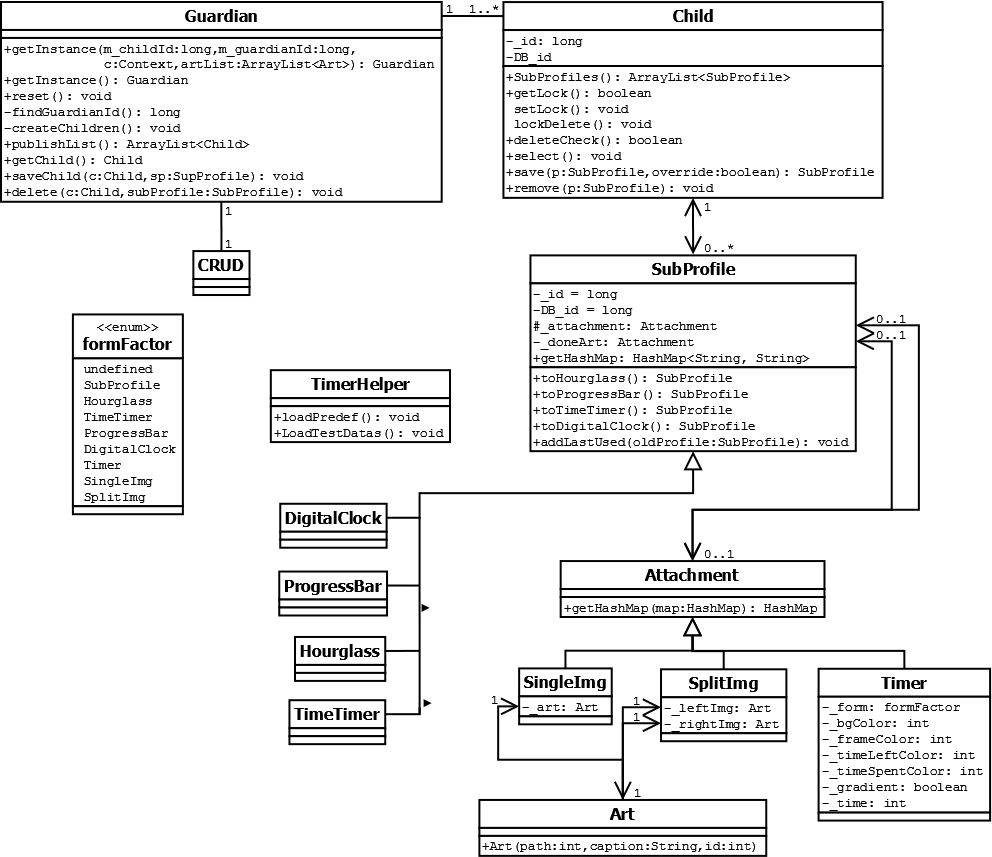
\includegraphics[scale=0.3]{Images/Implementation/classdiagram.png}
	\caption{Dependecy diagram of WOMBAT projects}
	\label{fig:classdiagram}
\end{figure}

\subsection{DrawLib}
%\textit{Beskrivelse af DrawLib, hvad indeholder DrawLib, services\\
%Beskrivelse af implementationen af DrawLib med kode eksempler\\
%Hvad er fordele ulemper for canvas frem for openGL}
\texttt{DrawLib} contains the functionality that draws timers according to the configuration selected in the main activity.
The main functionality in the \texttt{DrawLib} is that it can be either full screen, if there is no timer or pictogram(s) attached, or it can be split screen if there is a timer or pictogram(s) attached.
This is done by creating the view layout programmatically instead of a static layout, figure \ref{code:backend_drawlib_singletimer} is an example of this functionality with a full screen timer, figure \ref{code:backend_drawlib_splittimer} is an example of the functionality with a split screen timer.
In both figures the method \texttt{genDrawView} is a method which returns the draw view, that matches the timer specified in customization, figure \ref{code:backend_drawlib_gendrawview} is a code example of \texttt{genDrawView}.

\begin{figure}[H]
\begin{lstlisting}
public void onCreate(Bundle savedInstanceState) {
	super.onCreate(savedInstanceState);	
	requestWindowFeature(Window.FEATURE_NO_TITLE);
	View main_layout = findViewById(android.R.id.content).getRootView();
	main_layout.setSystemUiVisibility(View.STATUS_BAR_HIDDEN);
	Guardian guard = Guardian.getInstance();
	SubProfile sub = guard.getSubProfile();

	// Get display size and store it in static variables
	WindowManager wm = (WindowManager) getSystemService(Context.WINDOW_SERVICE);
	Display disp = wm.getDefaultDisplay();
	frameHeight = disp.getHeight();
	frameWidth = disp.getWidth();				

	if (sub.getAttachment() == null) {
		/* Set the drawing class (which extends View) as the content view */
		View v = genDrawView(sub,frameWidth);
		v.setKeepScreenOn(true);
		setContentView(v);
	} 
...
}
\end{lstlisting}
\caption{Code snippet of how \texttt{DrawLib} sets just one time \texttt{View}.}%
\label{code:backend_drawlib_singletimer}%
\end{figure}

\begin{figure}[H]%
\begin{lstlisting}
LinearLayout frame = new LinearLayout(this);
frame.setKeepScreenOn(true);
GradientDrawable gd = new GradientDrawable(GradientDrawable.Orientation.TOP_BOTTOM, new int[] {sub.bgcolor, 0xFF000000});

...

switch(sub.getAttachment().getForm()){
case Timer:
	frameWidth = frameWidth/2;
	
	firstView = genDrawView(sub, frameWidth);
	frame.addView(firstView, frameWidth, frameHeight);
	
	secondView = genDrawView(sub.getAttachment().genSub(), frameWidth);
	frame.addView(secondView, frameWidth, frameHeight);
	break;
case SingleImg:
	...
case SplitImg:
	...
}

setContentView(frame);
\end{lstlisting}
\caption{Code snippet of how \texttt{DrawLib} sets two timers in one \texttt{View}}%
\label{code:backend_drawlib_splittimer}%
\end{figure}

\begin{figure}[H]%
\begin{lstlisting}
private View genDrawView(SubProfile sub, int frameWidth) {
	switch (sub.formType()) {
	case ProgressBar:
		return new DrawProgressBar(getApplicationContext(), sub, frameWidth);
	case Hourglass:
		return new DrawHourglass(getApplicationContext(), sub, frameWidth);
	case DigitalClock:
		return new DrawDigital(getApplicationContext(), sub, frameWidth);
	case TimeTimer:
		return new DrawWatch(getApplicationContext(), sub, frameWidth);
	default:
		return null;
	}
}
\end{lstlisting}
\caption{Code snippet of the \texttt{genDrawView}, which generates the draw \texttt{View} matching the timer}%
\label{code:backend_drawlib_gendrawview}%
\end{figure}

\subsubsection*{Canvas and OpenGL comparision}
\label{subsection:compare}
%\textit{Hvad er fordelen ved at vælge canvas frem for openGL og hvorfor har vi valgt canvas?}
The timers in \texttt{DrawLib} are drawed with the Android \texttt{Canvas} object, this could have been done by creating and modelling an object in OpenGL.
The major difference between the two approaches is that OpenGL is used to draw three dimensional objects and Android \texttt{Canvas} draws in two dimensions.
Drawing on a canvas is like drawing on coordinates, while drawing in OpenGL varies in the way that it will be drawn in triangles.
Since all timers in WOMBAT can be modelled in two dimensions, the benefits of OpenGL compared to \texttt{Canvas} is that one would be able to move the camera around, change the zoom, or change the lighting in OpenGL.\\
\\

%The timers
%\textit{Introduktion til tegninger med canvas i Android\\
%Beskrivelse af implementationen af timere og hvordan bevægelser er udregnet\\
All timers are classes which inherits the \texttt{View} class, this class draw in a method called \texttt{onDraw}, \texttt{onDraw} is called when the class is initialized and afterwords when the method \texttt{invalidate()} is invoked.
The timers draw inside the \texttt{onDraw} method, as seen in figure \ref{code:backend_drawlib_onDraw}.

\begin{figure}[H]%
\begin{lstlisting}
protected void onDraw(Canvas c) {
	super.onDraw(c);
	
	... // Initialization of time + Draw Background and frame

	/* Draw the backgroundcolor inside the frame */
	paint.setColor(background);
	r.set(r.left + 2, r.top + 2, r.right - 2, r.bottom - 2);
	c.drawRect(r, paint);

	/* Draw the timespent color (on the right) on top of the timeleft */
	paint.setColor(timespent);
	r.set(left + 3, top + 3, left + width - 3, top + height - 3);
	c.drawRect(r, paint);

	if (endTime >= System.currentTimeMillis()) {
		timenow = endTime - System.currentTimeMillis();
		double percent = (timenow) / totalTime;

		paint.setColor(timeleft2);
		r.set((int) ((left + 3) + ((width - 5) * (1-percent))), top + 3, (left + 3) + width - 5, top
				+ height - 3);
		c.drawRect(r, paint);

		/* Draw the gradient color */
		...

		/*************** IMPORTANT ***************/
		/* Recalls Draw! */
		invalidate();
	} else {
		paint.setColor(timespent);
		r.set(left + 3, top + 3, left + width - 3, top + height - 3);
		c.drawRect(r, paint);
	}
}
\end{lstlisting}
\caption{Code snippet of the \texttt{onDraw} method of the progress bar.}%
\label{code:backend_drawlib_onDraw}%
\end{figure}

%Optimering af timere og de problemer vi løb ind i under vejs (canvas til bitmap og systemtimer)}
Drawing can be time consuming, so to optimize the timers, the background and frame is painted and stored as a bitmap file at the initialization of the drawing, seen in \autoref{code:drcode:drawlib_bitmap}.
The stored bitmap can then be redrawn on the canvas without having to be recalculated, this is specially useful when drawing the digital watch since all numbers has to be redrawn every time the view is evaluated.
With the bitmap it is possible to draw the numbers once and then blank out the lines not needed when evaluating.

\begin{figure}%
\begin{lstlisting}
/* Initialize a bitmap with the "standard" drawings */
bitmap = Bitmap.createBitmap(frameWidth, frameHeight, Bitmap.Config.ARGB_8888);
Canvas c = new Canvas(bitmap);

/* Fill the canvas with the background color */
...

y = (frameHeight - numHeight) / 2;

/* Draw first number */
x = numWidth/2 + numWidth;
c.drawPath(drawNumberPath(8, x, y), paint);

/* Draw second number */
x = numWidth/2 + numWidth * 2 + (numSpace);
c.drawPath(drawNumberPath(8, x, y), paint);

...
\end{lstlisting}
\caption{Code snippet of how the background and frame is stored as a bitmap.}%
\label{code:drcode:drawlib_bitmap}%
\end{figure}